\documentclass[11pt]{article}

\usepackage{times}
\usepackage[utf8]{inputenc}
\usepackage[T1]{fontenc}
\usepackage[english]{babel}
\usepackage{amssymb}
\usepackage{parskip}
\usepackage{url}
\usepackage{graphicx}

\begin{document}

\title{COMP512 - Distributed Systems \\ Assignment 1}
\author{
  Vincent Foley-Bourgon <vincent.foley-bourgon@mail.mcgill.ca> \\
  Carol Morneau <carol.morneau@mail.mcgill.ca>
}
\date{September 2013}

\maketitle

\section{Compilation and execution}

The whole system can easily be built with a single command:


\begin{verbatim}
$ make
\end{verbatim}

Running {\it make} in the root folder of the project will compile
all the different compononents of the project (middleware, client,
resource managers).

The different components can be started by using the helper {\it
  launcher.py} script in the root folder of the project.  The basic
syntax of the script is as follows:


\begin{verbatim}
./launcher.py <component> <tcp|rmi> <port> <extra args>
\end{verbatim}

The component is any of:

\begin{itemize}
\item middleware
\item client
\item customer
\item car
\item flight
\item hotel
\end{itemize}

You can select if you want the component to use the TCP protocol or
the RMI protocol.  Note that you cannot mix-and-match components of
different protocols (e.g. a TCP client cannot communicate with a RMI
middleware).

The port parameter lets you select on which port the middleware and
resource managers should listen on.  For the client, the port
parameter is the port of the middleware that it should connect to.

Finally, you can specify extra arguments to be passed to the
component.  Thw following components require extra arguments:

\begin{itemize}
\item client: requires the hostname of the middleware
\item customer: requires the hostname and port of the middleware.  The
  syntax is {\it host:port}.
\item middleware: requires the hostnames and ports of all resource
  managers.  The syntax is {\it backend=host:port}.  For example,
  specifying the customer resource manager location is done with {\it
    customer=localhost:9000}.
\end{itemize}




\section{TCP}

This section describes in some details the architecture and
implementation details of the TCP implementation of the system.


\subsection{Compononents}

The system is split into 6 distinct components:

\begin{itemize}
\item Client
\item Middleware
\item Car manager
\item Customer manager
\item Flight manager
\item Hotel manager
\end{itemize}

The middleware is the central hub of all inter-component
communication; at no point do the client or any manager directly
communicate with each other (see Figure \ref{fig:tcp}).


\begin{figure}[h]
  \begin{center}
    \caption{Architecture of TCP system \label{fig:tcp} }
    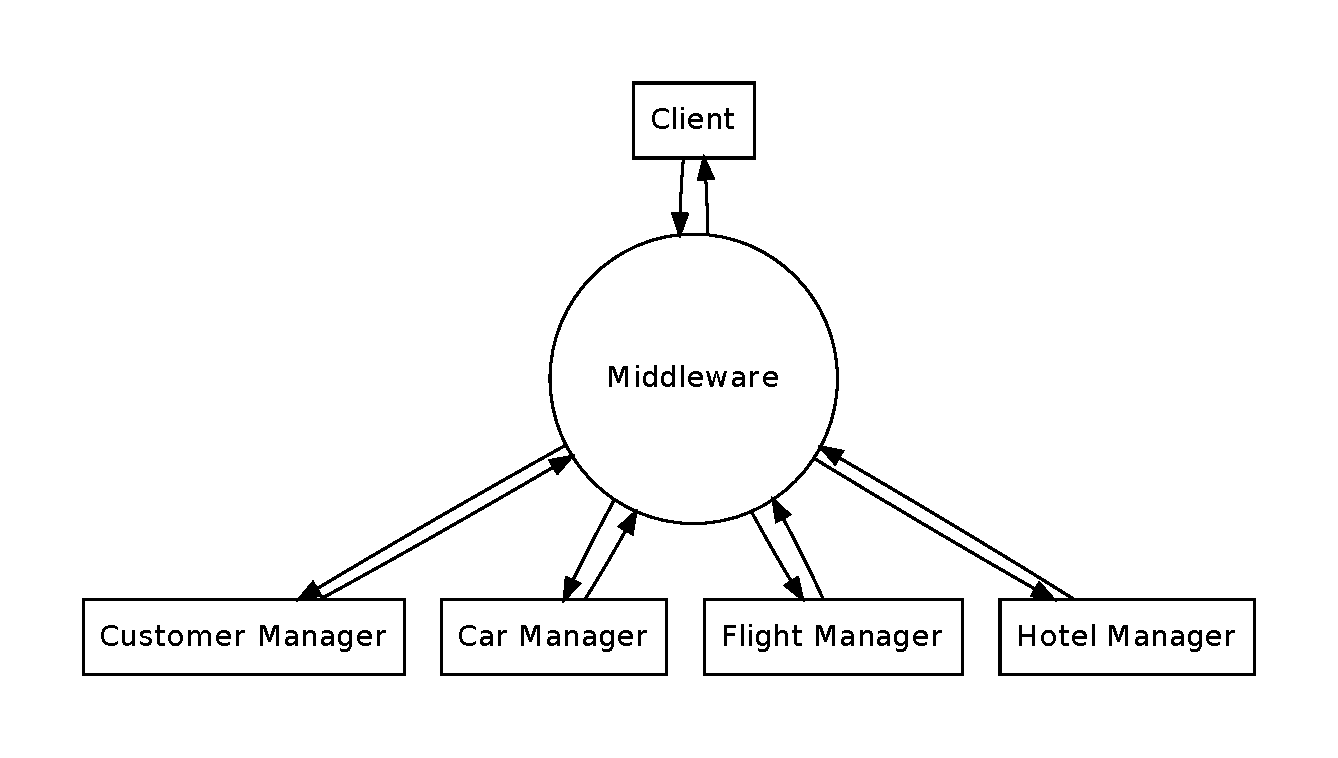
\includegraphics[scale=0.4]{tcp-diagram.pdf}
  \end{center}
\end{figure}

\subsubsection{Client}

The client is started by specifying the hostname and port of the
middleware server.  A connection is {\bf not} established as soon as
the client is started.  Instead, of a long-lived connection between
the client and the middleware, we have opted for making many
short-lived connections.  When a command is entered in the client,
only then is a connection established to the middleware, the command
is sent, and as soon as a response is received, the connection is
terminated.  There are two direct consequences to this design
decision:

\begin{itemize}
\item We can restart the server without having to restart the client.
\item The resources of the servers can be used to process actual
  commands instead of maintaining idle connections.
\end{itemize}

Commands are sent from the client to the middleware in
{\it ArrayList<String>} form.  Only the {\it help} and {\it quit}
commands are processed without accessing the middleware server.

\subsubsection{Middleware}

The middleware really is the nervous center of the system; it receives
the commands from the client and dispatches them to the appropriate
resource managers.  When it is started, the hostname and port of all
resource managers are given as arguments to the middleware.

The middleware receives commands from the client as {\it
  ArrayList<String>}; it dispatches to the appropriate manager by
inspecting the first item of the list, the command name.  Commands are
dispatched according to the following rules:


\begin{itemize}
\item If the command name contains the string {\it ``car''}, the
  message is forwarded to the Car Manager;
\item If the command name contains the string {\it ``customer''}, the
  message is forwarded to the Customer Manager;
\item If the command name contains the string {\it ``flight''}, the
  message is forwarded to the Flight Manager;
\item If the command name contains the string {\it ``room''}, the
  message is forwarded to the Hotel Manager;
\item If the command name is exactly {\it ``itinerary''}, the message
  is broken up into multiple messages and sent to the appropriate
  managers.
\end{itemize}

The middleware maintains a thread pool; whenever a connection to a
resource manager needs to be made, a thread is picked from that pool.
This allows the middleware to send off work and be immediately ready
to receive more connections from other clients.  Once the middleware
receives a response from a manager, it inspects the message for extra
operations to be performed on other managers (i.e. reservations need
to access a resource manager and the customer manager).  Once all work
has been done, the result of the command is sent back to the user.

\subsubsection{Resource Managers}

The resource managers for cars, flights and hotel are virtually
identical, so they are discussed together in this section.

The resource managers are started by specifying a listening port.
They do not know about the middleware directly.  They all maintain
thread pools.

When a request comes in, the resource manager will launch a new task
in a thread and listen for more connections.  The task will inspect
the message (an {\it ArrayList<String>}) and execute the correct
operation.


\begin{itemize}
\item {\it newitem}: a new item\footnote{item is used as a generic
    term for car, flight and room} is added to the hash table.
  Returns true if the operation succeeded, false otherwise.
\item {\it deleteitem}: an item is deleted from the hash table.
  Returns true if the item was delete, false if the item does not exist.
\item {\it queryitem}: returns the number of available items, 0 if the
  item does not exist.
\item {\it queryitemprice}: returns the price of the specified item, 0
  if the item does not exist.
\item {\it reserveritem}: returns a {\it ReservedItem} object if the
  reservation succeeded, {\it null} if it failed (i.e. no more
  available items)
\item {\it cancelitem}: cancels a reservation for an item.  Returns
  true if the cancellation succeeded, false if there was no
  reservation for the item.
\end{itemize}


\subsubsection{Customer Manager}

The customer manager is similar to the other resource managers, except
that it is the only resource manager that has direct knowledge of the
middleware.  This is not strictly necessary, but it helps make the
system simpler.  More details on this are given below.

The customer manager is started by specifying its localport and the
host and port of the middleware.  Like other resource managers, the
customer manager maintains a thread pool and dispatches to the correct
method based on the command name.


\begin{itemize}
\item {\it newcustomer}: create a new customer with a randomly-chosen
  id; return the id.
\item {\it newcustomer}: create a new customer with a specific id;
  return true if the operation succeeded, false if the id already exists.
\item {\it querycustomer}: return the bill for the customer; the empty
  string is returned if the client doesn't exist.
\item {\it deletecustomer}: remove the customer from the hash table
  and cancel all his reservations.
\end{itemize}

The command {\it deletecustomer} is complex enough to warrant extra
information.  When this command comes in, the customer is immediately
removed.  This avoid other clients making reservations for the
customer. Afterward, messages are sent to the middleware (in the same
format as the client would send them) to cancel the reservations for
the customer.

This explains why the customer manager knows about the middleware; it
can reuse the same communication protocol as the client to cancel
reservations.  If we wanted the customer manager to be unaware of the
middleware, we would need to do the extra communication through other
means, such as returning to the middleware a result containing a list
of the reservations to cancel.

\subsection{Message data structures}

There are two basic data structures used to transmit commands and
result back and forth in the system.

\subsubsection{Requests}

Requests (client commands) are transmitted as an {\it
  ArrayList<String>}.  This representation is not very rich, but is
sufficient at the moment for our needs.  If time had allowed it, a
representation using one class per message type, with a common
interface would've been a better design decision.

\subsubsection{Results}

Commands can return different results:

\begin{itemize}
\item Some commands (e.g. {\it newcar}) return true for success and
  false for failure
\item Some commands (e.g. {\it querycar}) return an integer
\item Some commands (e.g. {\it querycustomer}) return a string
\item Reserve commands return a {\it ReservedItem} object
\end{itemize}

To satisfy the Java type system, a new serializable class, {\it
  Result}, containing fields of types boolean, integer, string and
{\it ReservedItem} was created.  Once a resource manager has finished
executing a command, the result is wrapped into a result and sent back
to the middleware.

\subsection{Error handling}

Commands are not validated on the client side before being sent to the
middleware and dispatched to the appropriate resource manager.  If an
exception occurs in the resource manager (e.g. the string for the
customer id is not a string representing a valid integer), the
exception is caught and a result containing false is sent back to the
client.  In an industrial system, we would probably prefer to validate
on the client that the command is well-formed, as well as return a
proper error code from the resource manager (in case someone manages
to bypass the client validation).


\end{document}
